\documentclass[bachelor, och, coursework]{SCWorks}
\usepackage{subfigure}
\usepackage{tikz,pgfplots}
\pgfplotsset{compat=1.5}
\usepackage{float}
\usepackage{cmap}
%\usepackage{titlesec}
\setcounter{secnumdepth}{4}
%\titleformat{\paragraph}
%{\normalfont\normalsize}{\theparagraph}{1em}{}
%\titlespacing*{\paragraph}
%{35.5pt}{3.25ex plus 1ex minus .2ex}{1.5ex plus .2ex}

\titleformat{\paragraph}[block]
{\hspace{1.25cm}\normalfont}
{\theparagraph}{1ex}{}
\titlespacing{\paragraph}
{0cm}{2ex plus 1ex minus .2ex}{.4ex plus.2ex}

% --------------------------------------------------------------------------%


\usepackage[T2A]{fontenc}
\usepackage[utf8]{inputenc}
\usepackage{graphicx}
\graphicspath{ {./images/} }
\usepackage{tempora}

\usepackage[sort,compress]{cite}
\usepackage{amsmath}
\usepackage{amssymb}
\usepackage{amsthm}
\usepackage{fancyvrb}
\usepackage{listings}
\usepackage{listingsutf8}
\usepackage{longtable}
\usepackage{array}
\usepackage[english,russian]{babel}

% \usepackage[colorlinks=true]{hyperref}
\usepackage{url}

\usepackage{underscore}
\usepackage{setspace}
\usepackage{indentfirst} 
\usepackage{mathtools}
\usepackage{amsfonts}
\usepackage{enumitem}
\usepackage{tikz}
\usepackage{minted}

\newcommand{\eqdef}{\stackrel {\rm def}{=}}
\newcommand{\specialcell}[2][c]{%
\begin{tabular}[#1]{@{}c@{}}#2\end{tabular}}

\renewcommand\theFancyVerbLine{\small\arabic{FancyVerbLine}}

\newtheorem{lem}{Лемма}

\begin{document}

\chair{теоретических основ компьютерной безопасности и криптографии}

\title{Машинное обучение и трейдинг}

\course{3}

\group{331}

\department{факультета КНиИТ}

\napravlenie{10.05.01 "--- Компьютерная безопасность}

\author{Никитина Арсения Владимировича}

\chtitle{д.ф.-м.н., доцент} 
\chname{М. Б. Абросимов}


\satitle{д.ф.-м.н., доцент}
\saname{М. Б. Абросимов}

\date{2022}

\maketitle

%-------------------------------------------------------------------------------------------

\tableofcontents

\intro
    В последнее время анализ курсов акций является немаловажной проблемой.
    Так различают фундаментальный анализ, основанный на финансовой и
    производственной деятельности компаний, а также на общей экономической
    обстановке выбранной сферы. Также определен технический анализ, который
    основан на прогнозировании изменения курсов в зависимости от
    закономерностей изменений цен в прошлом в аналогичных обстоятельствах.

    Таким образом, в данной работе будет рассмотрена концепция технического
    анализа, его основные методы, инструменты, а также будет разработан
    детерминированный алгоритм нахождения технических фигур технического
    анализа.
    
    Более 150 лет торговые залы Чикагской фондовой биржи были местом проведения
    торговых сделок покупки и продажи.

    Вплоть до 1997 года более 10 тысяч людей торговали в общих залах Чикагских
    бирж (в так называемых <<биржевых ямах>>). Позднее, в том же году появилась
    торговля с помощью компьютеров. Сейчас только около 10\% трейдеров
    продолжают торговать в биржевых залах (остальные 90\% торгуют с
    компьютеров) \cite{HIST}.

    Несложно догадаться, что большинство трейдеров, использующих в качестве
    основного инструмента заработка компьютер, пользуются также различными
    вспомогательными средствами, обеспечивающие им уверенность в своих
    действиях.

    Итак, одним из средств, помогающих выполнять анализ поведения котировок
    акций, является технический анализ и, в частности, нахождение и анализ
    технических фигур.

\defabbr
    Перед анализом теоретической составляющей машинного обучения и технического
    анализа в трейдинге, стоит ввести ряд терминов и определений, являющихся
    основой для понимания работы алгоритмов поиска технических фигур, а также
    для определения основных составляющих трейдинга.

    \textit{Трейдинг} "--- покупка и продажа акций компаний с целью заработка на
    ежедневном демпинге цен. Трейдеры внимательно следят за краткосрочными
    колебаниями цен на эти акции, а затем пытаются купить подешевле и продать
    подороже. Этот краткосрочный подход отличает биржевых трейдеров от
    традиционных инвесторов фондового рынка, которые склонны работать в
    долгосрочной перспективе.

    \textit{Технический анализ} "--- это торговая дисциплина, используемая для
    оценки инвестиций и выявления торговых возможностей путем анализа
    статистических тенденций, полученных в результате торговой деятельности,
    таких как движение цены и объем. В отличие от фундаментального анализа,
    который пытается оценить стоимость ценной бумаги на основе результатов
    бизнеса, таких как продажи и прибыль, технический анализ фокусируется на
    изучении цены и объема.

    \textit{Фигура технического анализа} "--- определенная закономерность подряд
    идущих значений курса акции, которая отображаются на графике и позволяют
    трейдеру получать определенные сигналы о том, как стоимость актива будет
    строиться в будущем.

    \textit{Волатильность} "--- финансовый показатель, отражающий то, как сильно
    меняется цена на актив или товар за короткий промежуток времени \cite{OPCIONS}.

    \textit{Искусственный интеллект} (англ. Artificial Intelligence) "---
    технология создания алгоритмов, лежащих в основе проектирования
    интеллектуальных машин и программ, способных имитировать деятельность
    человека.

    \textit{Нейронная сеть (нейросеть)} (англ. Neural Network) "---
    математическая модель, чаще всего имеющая программную интерпретацию, сутью
    которой является реализация деятельности, похожей на деятельность
    биологических нейронных сетей. Нейронная сеть используется при создании
    какого-либо из алгоритмов искусственного интеллекта и состоит из
    совокупности нейронов, соединенных между собой связями. 

    \textit{Признак} (англ. Feature) "--- каждый отдельный элемент информации,
    включаемый в представление о каком-либо анализируемом объекте.

    \textit{Машинное обучение} (англ. Machine Learning) "--- область науки об
    искусственном интеллекте, которая изучает способы создания алгоритмов,
    которые могут обучаться (развиваться).


\section{Теоретическая часть}

    \subsection{Временной ряд}

        \textit{Временной ряд} — это определенные данные, собранные в разные
        моменты времени, графиком которого является значение времени по оси
        абсцисс и значение наблюдаемой величины в текущий момент времени по оси
        ординат \cite{wei2006time}.

        Временной ряд может иметь детерминированный компонент в определенный
        момент времени, тогда говорят, что данные временного ряда имеют
        временной тренд.
    
        Временные тренды в данных временных рядов также имеют значение для
        тестирования и моделирования. Надежность модели временных рядов зависит
        от правильного определения и учета временных тенденций.
    
        Определить, наличие временного тренда на графике можно с помощью
        проведения возрастающей (убывающей) линии и выявления сосредоточения
        значений наблюдаемой величины в окрестности этой линии.

        \begin{figure}[H]
            \centering
            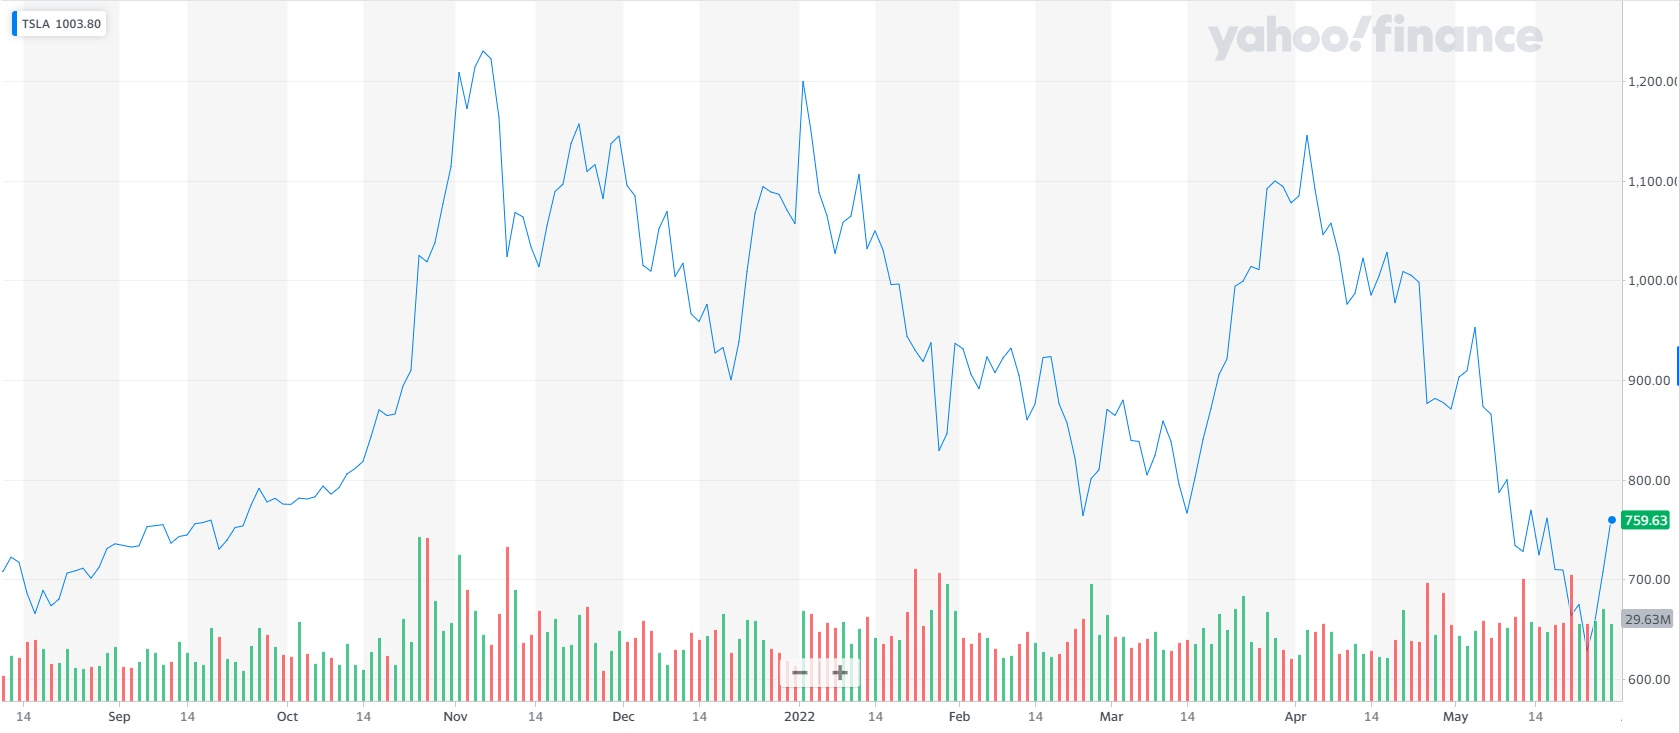
\includegraphics[width=0.8\textwidth]{pic/timeseries.jpg}
            \caption{Пример временного ряда}
        \end{figure}


        \subsection{Основы технического анализа}

            \subsubsection{Японская свеча}

            Графики свечей — наиболее популярная в Японии и самая древняя форма
            технического анализа. <<Японские свечи>> появились раньше, чем
            штриховые графики и графики «крестики-нолики». Японцы осознали
            важность технического анализа давным-давно. Они первыми стали
            торговать фьючерсами. В середине XVII в. они торговали <<пустыми>>
            рисовыми контрактами (рисом, которого еше не было, "--- иначе
            говоря, рисовыми фьючерсами) \cite{wagner1993trading}.

            Японская свеча состоит из следующих компонентов: 
            \begin{enumerate}
                \item Open (цена открытия) "--- цена на начало периода.
                \item Close (цена закрытия) "--- цена на конец периода.
                \item High "--- максимальная цена в течение периода.
                \item Close "--- минимальная цена в течение периода.
            \end{enumerate}

            \begin{figure}[H]
                \centering
                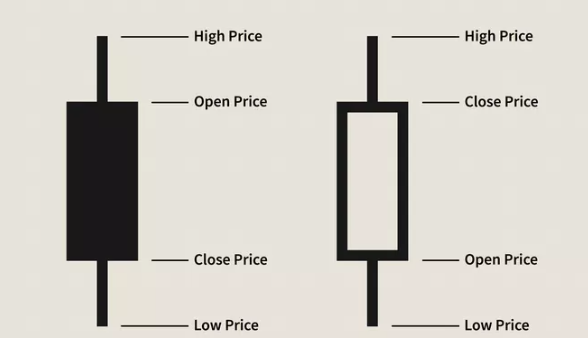
\includegraphics[width=0.8\textwidth]{pic/candlestick.png}
                \caption{Японская свеча}
            \end{figure}

            Для того, чтобы можно было отрисовать график акций, требуется
            использовать один из показателей японской свечи. В данной работе
            далее используется показатель $Close$.

            \subsubsection{Определение тенденции с помощью макисмумов и минимумов}

            В качестве одного из стандартных методов определения тенденции
            повышения можно рассмотреть последовательности более высоких
            максимумов и более низких минимумов \cite{schwager1995technical}.    

            Итак, тенденция повышения является ненарушенной ровно до тех пор,
            пока зафиксированный предыдущий относительный минимум не будет
            пробит, то есть не образуется новый минимум. Если такое происходит,
            то делается вывод о том, что тенденция закончилась или же в скором
            времени это произойдет.

            Аналогично можно определить и понижающую тенденцию как
            последовательность более низких минимумов и более низких максимумов.
            Понижающая тенденция является ненарушенной до тех пор, пока
            зафиксированный предыдущий максимум не пробит. Если же наблюдается
            пробитие максимума, то возможно понижающая тенденция подходит к
            своему завершению.

                \begin{figure}[H]
                    \centering
                    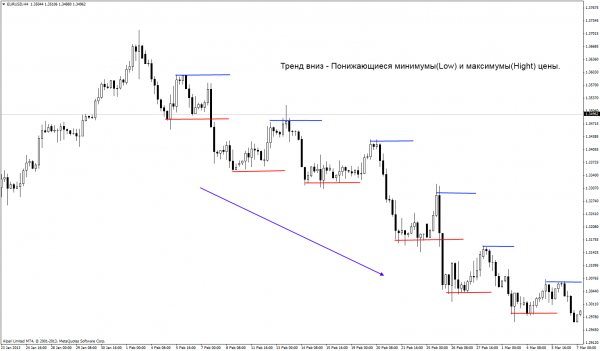
\includegraphics[width=0.8\textwidth]{pic/trand.png}
                    \caption{Пример нисходящего тренда}
                \end{figure}

            \subsubsection{Линия роста (падения)}
            Кумулятивная дневная линия роста / падения является одним из
            наиболее известных индикаторов разброса рынка и часто используется
            для обнаружения дивергенции (расхождения) с одним из свободных
            индексов рынка. Как правило, кумулятивная линия роста (падения)
            вычисляется как скользящая сумма чистого количества растущих акций.
                
            Вычисление значений линии роста (падения) проводится в два этапа:
                \begin{enumerate}
                    \item Вычисление разности между количеством растущих и
                    количеством падающих акций с сохранением знака результата.
                    Полученное значение также называется \textit{чистым
                    количеством растущих акций}.
                    \item Прибавить вычисленную сумму за данный день к значению
                    накопленной суммы ежедневных количеств \textit{растущих
                    акций}.
                \end{enumerate}

            Также предлагается приступать к вычислению кумулятивной скользящей
            только после проведения нормализации дневных данных по формуле:
                \begin{center}
                    $N = \frac{A - D}{A + D} $, 
                \end{center}
                где $N$ "--- отношение чистого количества растущих акций к
                общему числу акций, показавших изменение цены, $A$ "---
                количество растущих акций, $D$ "--- количество падающих акций.

        \subsection{Перцептрон как один из методов реализации нейронных сетей}
        
        Типичным примером модели глубокого обучения является глубокая сеть
        прямого распространения, или многослойный перцептрон (МСП). Многослойный
        перцептрон "--- это математическая функция, отображающая множество
        входных значений на множество выходных. Эта функция является композицией
        нескольких более простых функций. Каждое применение одной математической
        функции можно рассматривать как новое представление входных данных.
        
        Глубина позволяет обучать многошаговую компьютерную программу. \\Каждый
        слой представления можно мыслить себе как состояние памяти компьютера
        после параллельного выполнения очередного набора инструкций. Чем больше
        глубина сети, тем больше инструкций она может выполнить последовательно.
        Последовательное выполнение инструкций расширяет возможности, поскольку
        более поздние инструкции могут обращаться к результатам выполнения
        предыдущих.
        
        Есть два основных способа измерить глубину модели. Первый оценивает
        архитектуру на основе числа последовательных инструкций, которые
        необходимо выполнить. Можно считать, что это длина самого длинного пути
        в графе, описывающем вычисление каждого выхода модели по ее входам. Как
        у двух эквивалентных компьютерных программ могут быть разные длины пути
        в зависимости от языка, на котором они написаны, так и одна и та же
        функциональность может быть изображена графами с разной длиной пути в
        зависимости от того, какие функции допускаются в качестве шагов. 

        При другом подходе, используемом в глубоких вероятностных моделях,
        глубиной модели считается не глубина графа вычислений, а глубина графа,
        описывающего связи концепций. В этом случае граф вычислений, выполняемых
        для вычисления представления каждой концепции, может быть гораздо
        глубже, чем граф самих концепций. Связано это с тем, что понятие системы
        о простых концепциях можно уточнять, располагая информацией о более
        сложных. Например, система ИИ, наблюдающая изображение лица, на котором
        один глаз находится в тени, первоначально может распознать только один
        глаз. Но, обнаружив присутствие лица, система может заключить, что
        должен быть и второй глаз. В таком случае граф концепций содержит только
        два слоя "--- для глаз и для лиц, тогда как граф вычислений содержит
        $2n$ слоев, если мы $n$ раз уточняем оценку каждой концепции при
        известной информации о второй.

        Поскольку не всегда ясно, какой из двух подходов – глубина графа
        вычислений или глубина графа вероятностной модели – более релевантен, и
        поскольку разные люди по-разному выбирают наборы примитивных элементов,
        из которых строятся графы, не существует единственно правильного
        значения глубины архитектуры, как не существует единственно правильной
        длины компьютерной программы. И нет общего мнения о том, какой должна
        быть глубина, чтобы модель можно было считать <<глубокой>>. Однако можно
        все-таки сказать, что глубокое обучение "--- это наука о моделях, в
        которых уровень композиции обученных функций или обученных концепций
        выше, чем в традиционном машинном обучении \cite{GF}.

        \subsection{Использование нейронных сетей для поиска фигур технического анализа}
        Существует целая теория распознавания изображений образов, являющаяся
        разделом кибернетики.

        Нейронные сети в рассматриваемой задачи могут дать преимущество в связи
        с тем, что они имеют афинную инвариантность к представляемым данным, в
        частности, к масштабу и углам смещения фигур технического анализа. Тогда
        данные отклонения можно считать шумом, с которым нейронная сеть, как
        правило умеет работать. 

        Одним из первых вопросов при использовании нейронной сети для нашей
        задачи является количество входов и подаваемая на них информация. Также
        важным моментом является выбор типа нейронной сети, ее параметром и
        методов обучения. Рассматриваемая проблема относится к классу задач
        классификации, а, значит, необходимо понять, к какой фигуре относится
        текущее поведение временного ряда.

        В качестве входной информации для нейронной сети можно использовать
        координаты начала отрезка, его окончания и угол наклона прямой. 

        Итак, для задачи о предсказании поведения текущего курса акций разумно в
        качестве нейросетевого ядра использовать многослойный перцептрон с
        обучением по методу обратного распространения ошибки. Данный тип
        нейронной сети хорошо зарекомендовал себя в задачах прогнозирования.

        На входы нейронной сети будут подаваться параметры нескольких подряд
        идущих отрезков. На выходе будут параметры следующего отрезка.
        
        Нейронные сети, безусловно, являются одним из методов поиска фигур
        технического анализа и предсказания поведения акций в зависимости от
        полученных результатов работы. В данной работе же рассматриваются
        детерминированные подходы которые пытаются выделить технические фигуры
        на заданном временном ряде и затем провести прогнозирование поведения
        ряда в зависимости от найденных фигур \cite{SHUMKOV}.


\section{Практическая часть}

    \subsection{Описание инструментов и библиотек программной реализации}

        % Python
        В виду своей удобности использования, простоты написания кода, а также
        различных дополнительных библиотек для анализа акций, в данной работе
        используется язык программирования Python. Простота применения Python
        для написания кода и возможность его отладки через такие пакетные
        менеджеры, как conda, упрощают обмен библиотеками и результатами
        исследований. Его экосистема библиотек для работы в сфере трейдинга,
        таких как NumPy, yfinance и Matplotlib, упрощают анализ результатов
        работы алгоритма, получение котировок акций с различной временной
        градацией.


        %Yahoo Finance
        Yfinance "--- популярная библиотека с открытым исходным кодом,
        разработанная Раном Арусси как средство доступа к финансовым данным,
        расположенным на ресурсе Yahoo Finance.

        Yahoo Finance предлагает обширный набор рыночных данных по акциям,
        облигациям, валютам и криптовалютам. Для удобства использования в данной
        библиотеке присутствует возможность получения отчетов и анализов данных,
        а также дополнительные параметры получаемых данных, что отличает его от
        ряда конкурентов.

        Также стоит отметить, что отличительной особенностью yfinance является
        то, что библиотека позволяет получить градуирование данных вплоть одной
        минуты. Однако, что данные за текущий день получить нельзя. Если
        требуется получить данные за день (то есть градуирование составляет по
        часам и меньше), то минимально возможная разница в днях с текущей датой
        составляет 60 дней.

        Получаемые данные представляют из себя $csv$-файл, в котором
        присутствуют вышеописанные элементы свечей: максимальная (минимальная)
        цена, открытие (закрытие) акции \cite{YFLIB}.

        %Matplotlib
        
        Matplotlib "--- это кроссплатформенная библиотека для визуализации
        данных и графического построения графиков для Python и NumPy. В данной
        работе использование библиотеки является необходимым для отображения
        котировок акций и найденных фигур технического анализа с предполагаемым
        ростом (падением) курса. По оси абсцисс будем брать градуирование даты,
        а по оси ординат будем использовать полученные с помощью yfinance
        котировки, используя поле $close$ \cite{tosi2009matplotlib}.


    \subsection{Программная реализация алгоритма}
    
    Детерминированная реализация поиска технических фигур на акциях будет
    состоять из нескольких этапов:
    \begin{enumerate}
        \item Выбор рассматриваемой акции.
        \item Получение котировок за определенный период.
        \item Нахождение экстремумов временного ряда.
        \item Итеративный проход по полученным значениям с проверкой условия
        попадания $k$ подряд идущих значений в некоторые допуски.
        \item Принятие решения о нахождении фигуры и прогноз дальнейшего роста
        или падения курса.
    \end{enumerate}
          
    
    Итак, для начала определимся, каким образом можно найти фигуры технического
    анализа путем сравнения подряд идущих значений с допусками. Для этого
    рассмотрим основные фигуры технического анализа и получим закономерности, по
    которым и будут проверяться условия попадания значений в результат.
    
        \subsubsection{Флаги и вымпелы}

        Флагами и вымпелами называются узкие и краткосрочные (например, от одной
        до трех недель) фазы консолидации внутри трендов. Фигура называется
        флагом, когда она ограничена параллельными линиями, и вымпелом, когда
        линии сходятся. 

        Флаги и вымпелы обычно отражают паузы в сильном тренде, а также зачастую
        направлены в сторону, противоположную основной тенденции. Иначе говоря,
        за этими моделями, как правило, следует движение цен в том же
        направлении, которое предшествовало их формированию.

        Пробой границы флага или вымпела может рассматриваться как подтверждение
        того, что тренд продолжается, и как сигнал к торговле в направлении
        тренда. 

        Значительный пробой за пределы флага или вымпела в направлении,
        противоположном ожидаемому, то есть против основной тенденции, может
        рассматриваться как сигнал потенциального разворота тенденции
        \cite{schwager1995technical}. 

    \begin{figure}[H]
        \centering
        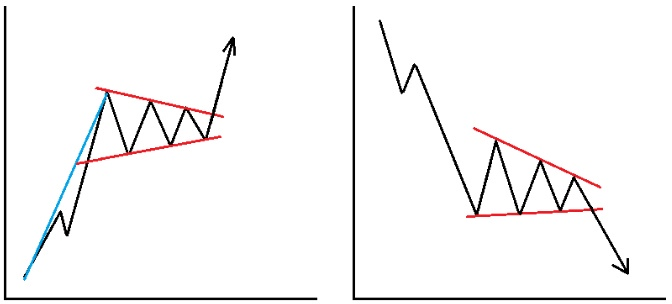
\includegraphics[width=0.8\textwidth]{pic/pennants.jpg}
        \caption{Восходящий и нисходящий вымпелы}
    \end{figure}

    Итак, как видно из левой части рисунка, формирование фигуры <<восходящий
    вымпел>> будет зависеть от 6-ти подряд идущих значений, причем нечетные
    значения должны убывать относительно друг друга, а четные значения "---
    возрастать. Также последнее нечетное значение должно быть гарантированно
    меньше последнего четного. Если до начала формирования восходящего вымпела
    временной ряд показывал рост, то фигура найдена и предполагаемое значение
    должно расти.

    Для фигуры <<нисходящий вымпел>> также будем проверять 6 подряд идущих
    значений, только нечетные значения должны убывать относительно друг друга, а
    четные значения должны быть равны между собой с учетом некоторого допуска.
    Последнее четное значение также должно быть меньше последнего нечетного.
    Если до начала формирования фигуры значения акций убывали, то после
    окончания формирования, тренд останется таким же.

    \begin{figure}[H]
        \centering
        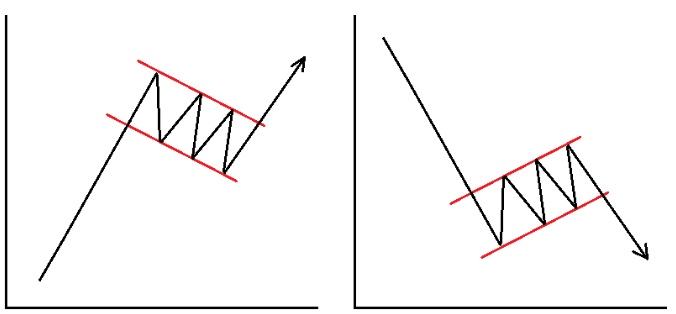
\includegraphics[width=0.8\textwidth]{pic/flags.jpg}
        \caption{Восходящий и нисходящий флаги}
    \end{figure}

    Теперь перейдем к рассмотрению восходящих и нисходящих флагов. Также, как и
    в случае с вымпелами потребуется сравнить между собой 6 подряд идущих
    значений временного ряда. Для того, чтобы сделать вывод о формировании
    флага, требуется, чтобы при соединении четных (нечетных) значений
    образовывалась прямая, причем полученные две прямые не должны пересекаться.
    Для этого требуется ввести определенный допуск и посчитать коэффициент
    прямой по формуле:
    \begin{center}
        $\frac{y_2 - y_1}{x_2 - x_1}$,
    \end{center}
    где в качестве значения знаменателя будем брать $1$, так как две соседние
    точки будут иметь разницу ровно один день. А в качестве числителя будем
    брать разницу между соседними значениями.
    
    Таким образом получим два коэффициента: $k_1, k_2$. Теперь вычтем один
    коэффициент из другого по модулю и сравним с некоторым допуском
    $\varepsilon$. Если $|k_1 - k_2| < \varepsilon$, то фигура найдена. Если
    полученные коэффициенты отрицательны и до этого тренд был возрастающим, то
    он сохранится. Если же коэффициенты положительны и тренд был нисходящим, то
    он также сохранится.

    \subsubsection{Прямоугольник}

    Фигура <<прямоугольник>> представляет своего рода канал, в пределах которого
    колеблется цена. Возникает, если котировки не в состоянии продолжить
    движение по тренду. Если движение по тренду останавливается на какое-то
    время, но при этом цена не в состоянии развернуться против тренда, то с
    большей вероятностью актуальная тенденция будет продолжена.

    \begin{figure}[H]
        \centering
        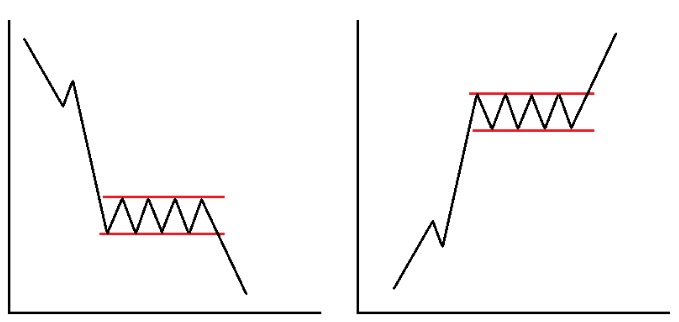
\includegraphics[width=0.8\textwidth]{pic/rectangles.jpg}
        \caption{Прямоугольник}
    \end{figure}

    Рассмотрим алгоритм нахождения прямоугольников на графике. Будем
    рассматривать 8 подряд идущих значений и сравнивать их с определенным
    допуском. Четные и нечетные значения должны быть примерно равны между собой,
    то есть $|y_i - y_{i + 2}|<\varepsilon$.
    
    Если до начала формирования фигуры тренд шел на понижение, то после
    окончания ее формирования он останется. Для возрастающего тренда ситуация
    аналогичная.

    \subsubsection{Ромб}

    Начало ромба возникает в конце импульсного движения по тренду. Цена
    затормаживается, после чего ее колебания постепенно возрастают, но
    происходят в пределах расходящегося треугольника (левая половина ромба).
    Затем происходит обратное "--- волатильность плавно снижается, и мы
    наблюдаем окончательное формирование ромба.

    Как и в случае с другими фигурами, объемы торгов являются отличным
    вспомогательным инструментом при определении границ и момента завершения
    ромба. Например, импульсный рост объемов возле границы ромба увеличивает
    вероятность завершения фигуры.

    \begin{figure}[H]
        \centering
        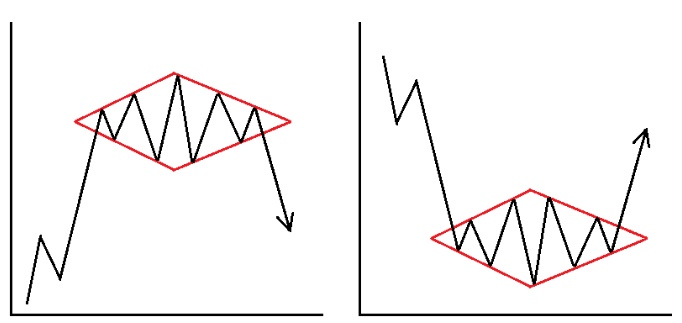
\includegraphics[width=0.8\textwidth]{pic/rhombuses.jpg}
        \caption{Ромб}
    \end{figure}
   
    Будем рассматривать 9 подряд идущих значений: первые 3 нечетных значения
    должны возрастать (в случае нахождения средней вершины ромба как точки
    перегиба в убывающий тренд, если же средняя вершина будет точной перегиба в
    возрастающий тренд, то будем учитывать первые 2 четных вершины как
    возрастающие), последние 2 нечетных значения должны убывать. Четные же
    вершины наоборот сначала должны убывать по значениям, а затем возрастать.
    Также стоит учитывать то, что значение средней вершины должно быть локальным
    максимумом (минимумом) среди всех подряд идущих. Таким образом, будет сделан
    вывод о формировании фигуры <<ромб>>.

    Если до начала формирования фигуры тренд шел на повышение и среднее значение
    ромба является локальным максимумом, то тренд после окончания формирования
    фигуры будет идти на понижение. Если же указанное значение является
    локальным минимумом, а тренд шел на понижение, то он развернется и пойдет на
    повышение.

    \subsubsection{Голова и плечи}
    <<Голова и плечи>> "--- одна из самых известных графических моделей.
    Формация <<голова и плечи>> представляет собой конфигурацию из трех вершин,
    причем средняя из них выше двух "--- предшествующей и последующей.
    Аналогичным образом, перевернутая <<голова и плечи>> представляет собой
    конфигурацию из трех впадин, причем средняя впадина ниже соседних. Данная
    фигура не считается завершенной, пока не пробита линия <<шеи>>. Более того,
    подлинная «голова и плечи» формируется только после того, как после пробоя
    <<линии шеи>> произошло значительное движение цен. Модели, которые похожи на
    <<голову и плечи>>, но не удовлетворяют последнему требованию, могут
    оказаться ложными \cite{colby2003encyclopedia}.
    
    \begin{figure}[H]
        \centering
        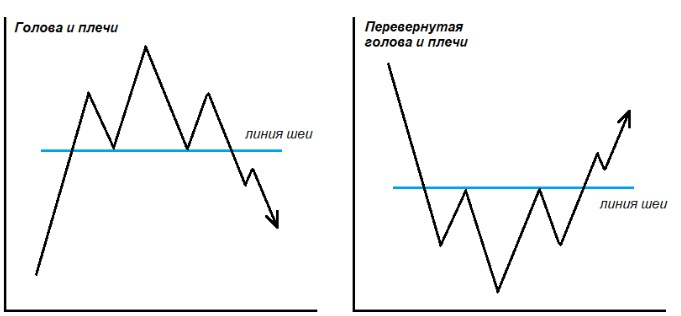
\includegraphics[width=0.8\textwidth]{pic/headshoulders.jpg}
        \caption{Голова и плечи}
    \end{figure}

    Итак, для того, чтобы найти данную фигуру, будем рассматривать 5 подряд
    идущих значений временного ряда. Первое значение должно быть строго большим
    второго значения, чтобы получилось <<левое плечо>>, причем тренд до начала
    фигуры должен быть возрастающим. Третье значение в случае не перевернутой
    фигуры должно быть максимальным из рассматриваемых. Аналогично, четвертое
    значение должно быть строго меньше пятого. Если все данные условия
    выполнены, то делается вывод о том, что сформировалась очередная фигура
    <<голова и плечи>> и, значит, тренд пойдет вниз.

    Перевернутая голова и плечи строится аналогично: второе значение строго
    больше первого, четвертое значение строго больше пятого и третье значение
    является минимальным из рассматриваемых. Тренд до образования фигуры
    убывающий, а, значит, после окончания формирования, должен пойти вверх.

    \subsection{Поиск экстремальных значений}
    Воспользуемся одним из методов технического анализа "--- поиск экстремальных
    значений котировок и составление нового графика на их основе. Для этого
    будем сравнивать подряд идущие значения $x_1, x_2, x_3$.

    Если $x_2 < x_3$ и $x_2 < x_1$, то точка $x_2$ будет являться экстремальным
    значением с дальнейшим восходящим трендом, начиная с точки $x_3$.

    Если же $x_2 > x_3$ и $x_2 > x_1$, то точка $x_2$ будет являться
    экстремальным значением с дальнейшим нисходящим трендом, начиная с точки
    $x_3$.

    Возьмем, например, акции Netflix за последние 5 лет и проверим работу
    рассматриваемого алгоритма.
    
    \begin{figure}[H]
        \centering
        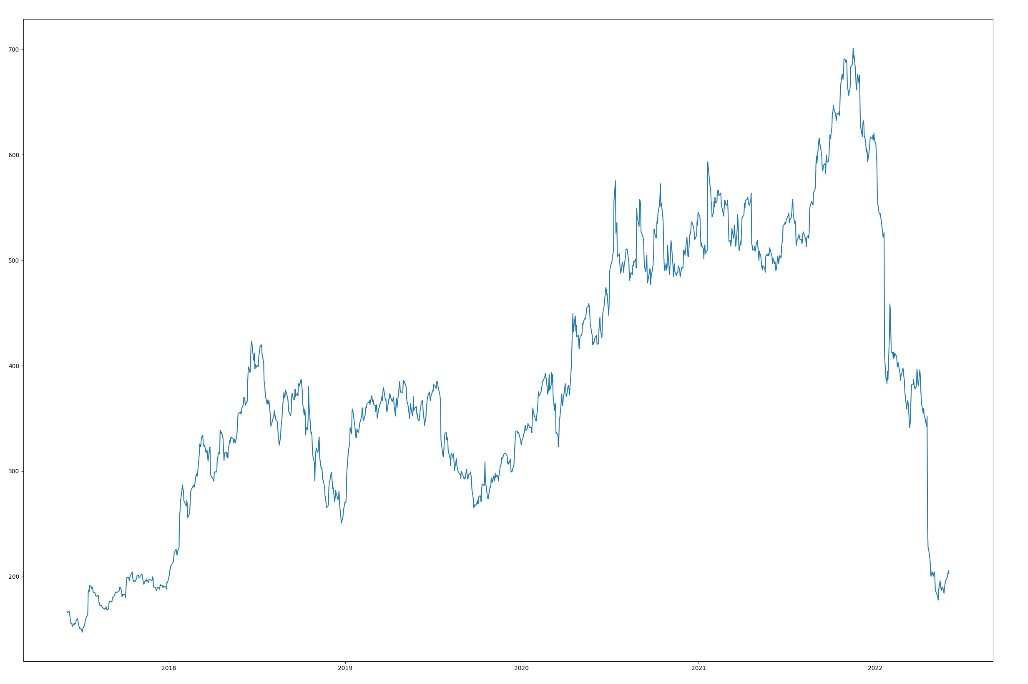
\includegraphics[width=0.8\textwidth]{pic/NetflixInitial.jpg}
        \caption{График акций Netflix}
    \end{figure}

    Всего было получено 1260 значений цен. Теперь воспользуемся алгоритмом
    получения экстремальных значений, а также аналогично изобразим временной
    ряд.
    
    \begin{figure}[H]
        \centering
        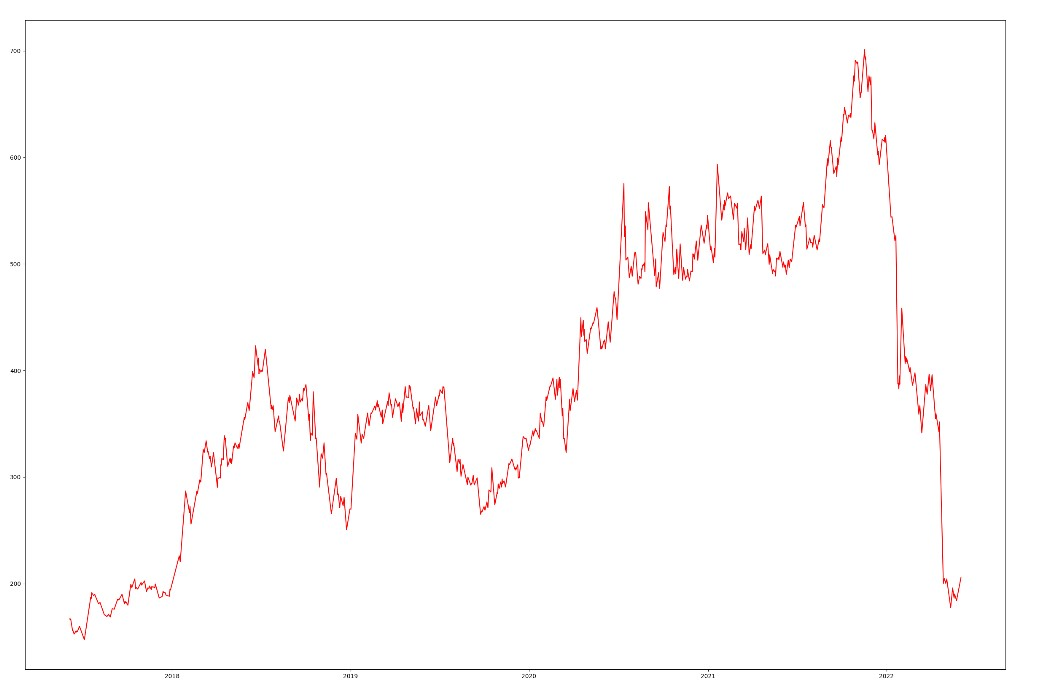
\includegraphics[width=0.8\textwidth]{pic/NetflixExtrema.jpg}
        \caption{График акций Netflix по экстремумам}
    \end{figure}
    
    После работы алгоритма, было получено 560 экстремальных значений.


    \subsection{Проверка работы алгоритма}
    Итак, перейдем к проверке работы алгоритма, а также к анализу получаемого
    результата нахождения технических фигур. Для этого сделаем анализ котировок
    четырех акций с высокой волатильностью, четырех с низкой волатильностью, а
    также возьмем в рассмотрение две котировки акций криптовалют. Затем сделаем
    вывод о том, какие из рассматриваемых акций поддаются техническому анализу,
    а также получим общий вывод по работоспособности алгоритма. Все акции будем
    рассматривать за последние пять лет, следовательно цены на акции будем брать
    с промежутком в один день \cite{YF}.
    
    На графике будем изображать работу алгоритма поиска экстремумов, а также
    будем наносить поверх графика экстремумов найденные фигуры с предполагаемым 
    дальнейшим ростом или падением курса.
    
    Для начала рассмотрим акции с высокой волатильностью.
    
    \subsubsection{Energy Focus}
    
    \begin{figure}[H]
        \centering
        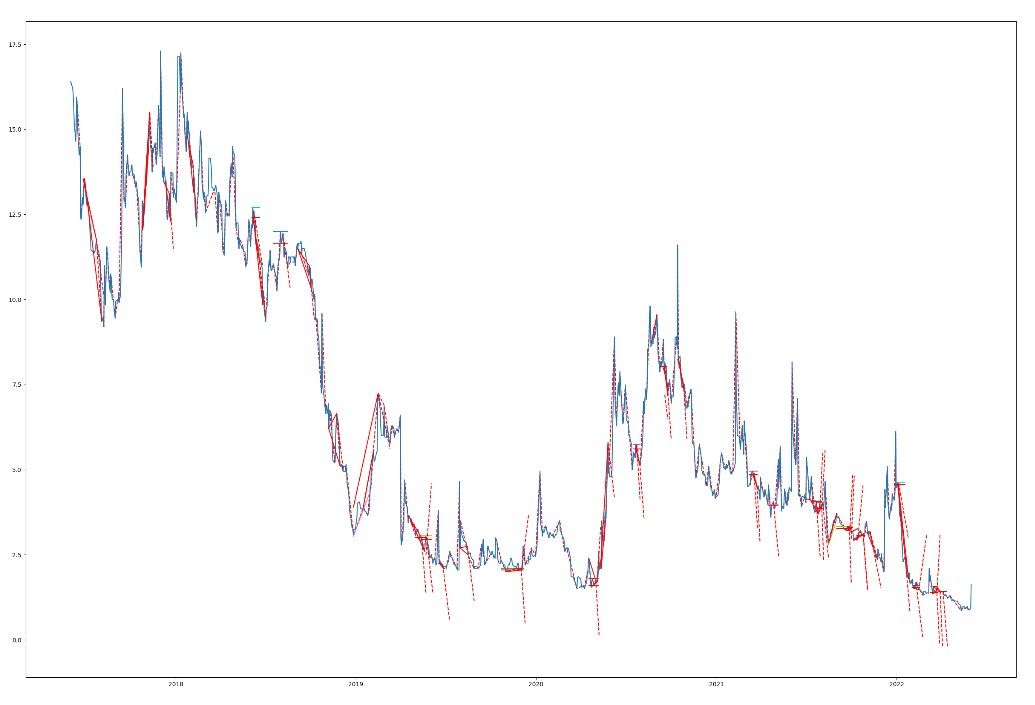
\includegraphics[width=0.8\textwidth]{pic/EFOI.jpg}
        \caption{График акций и технические фигуры Energy Focus}
    \end{figure}
   
    \begin{table}[!hbt]
        \centering
        \begin{tabular}{|l|c|c|c|}
        \hline
        Фигура                      & \multicolumn{1}{l|}{Количество найденных} & Совпадение & Доля  \\ \hline
        Вымпел                      & 2                                         & 2          & 0.023 \\ \hline
        Нисходящий флаг             & 2                                         & 2          & 0.023 \\ \hline
        Восходящий флаг             & 4                                         & 3          & 0.047 \\ \hline
        Прямоугольник               & 3                                         & 3          & 0.035 \\ \hline
        Нисходящий ромб             & 1                                         & 1          & 0.012 \\ \hline
        Восходящий ромб             & 0                                         & 0          & 0     \\ \hline
        Голова и плечи              & 2                                         & 2          & 0.023 \\ \hline
        Перевернутые голова и плечи & 3                                         & 3          & 0.035 \\ \hline
        \end{tabular}
        \end{table}

    Исходя из полученных данных, можно сделать вывод, что для акций Energy Focus
    не было найдено достаточное количество технических фигур для проведения 
    анализа, но для большинства найденных фигур предполагаемый курс акций 
    совпадал с действительным.


    \subsubsection{Yandex}
    
    \begin{figure}[H]
        \centering
        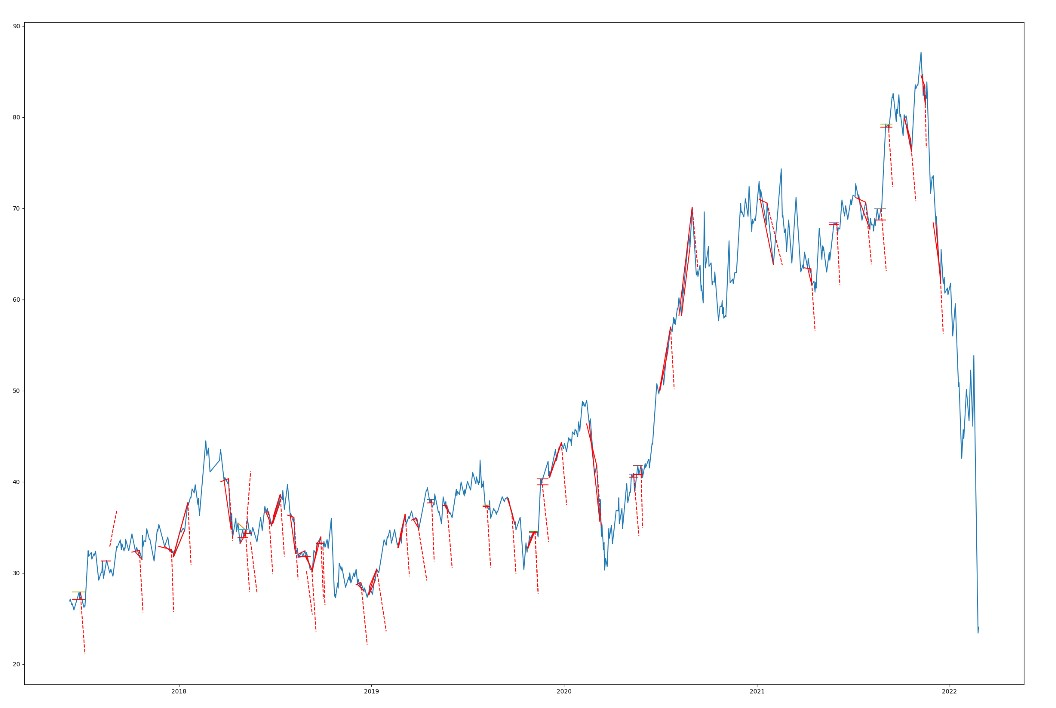
\includegraphics[width=0.8\textwidth]{pic/Yandex.jpg}
        \caption{График акций и технические фигуры Yandex}
    \end{figure}
   
    \begin{table}[!hbt]
        \centering
        \begin{tabular}{|l|c|c|c|}
        \hline
        Фигура                      & \multicolumn{1}{l|}{Количество найденных} & Совпадение & Доля  \\ \hline
        Вымпел                      & 1                                         & 1          & 0.013 \\ \hline
        Нисходящий флаг             & 0                                         & 0          & 0     \\ \hline
        Восходящий флаг             & 6                                         & 6          & 0.078 \\ \hline
        Прямоугольник               & 0                                         & 0          & 0     \\ \hline
        Нисходящий ромб             & 0                                         & 0          & 0     \\ \hline
        Восходящий ромб             & 0                                         & 0          & 0     \\ \hline
        Голова и плечи              & 3                                         & 3          & 0.039 \\ \hline
        Перевернутые голова и плечи & 1                                         & 1          & 0.013 \\ \hline
        \end{tabular}
        \end{table}

    В данный момент Yandex относится к компаниям, имеющим акции с 
    высокой волатильностью. Исходя из полученных данных, можно сделать вывод
    что данные котировки можно отнести к неподдающимся техническому анализу, 
    так как фигур <<прямоугольник>> и <<ромб>> вообще не было найдено, а
    остальные фигуры были найдены в недостаточном количестве.
    

    \subsubsection{Rectruiter.com Group}
    
    \begin{figure}[H]
        \centering
        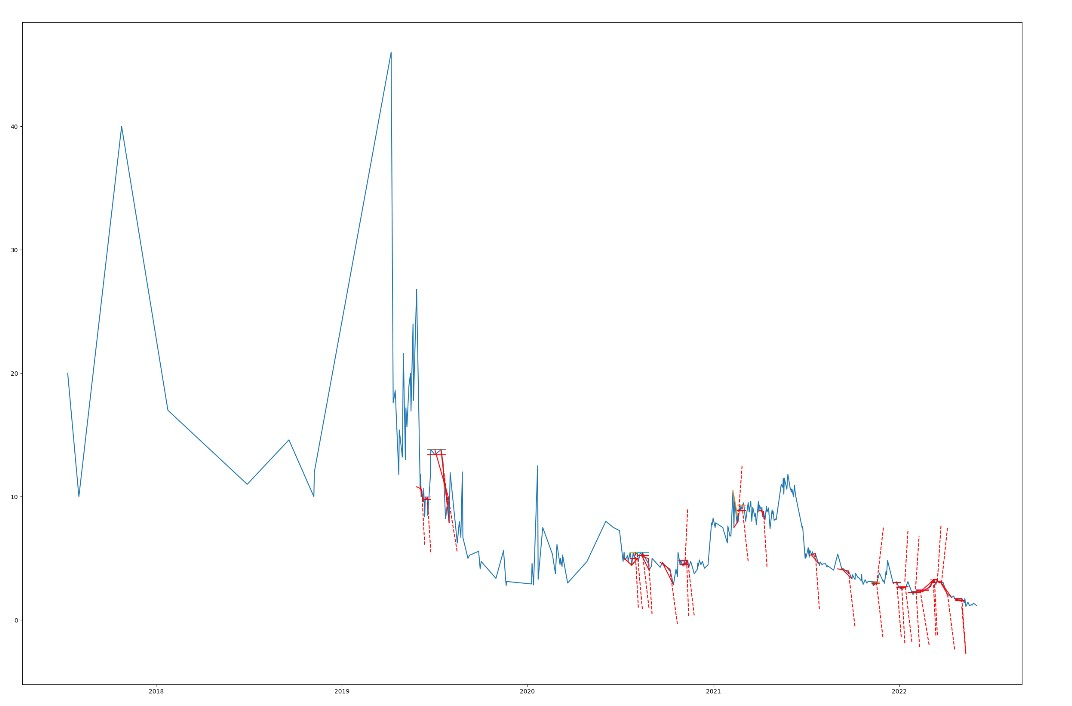
\includegraphics[width=0.8\textwidth]{pic/RCRT.jpg}
        \caption{График акций и технические фигуры Recruiter.com}
    \end{figure}
   
    \begin{table}[!hbt]
        \centering
        \begin{tabular}{|l|c|c|c|}
        \hline
        Фигура                      & \multicolumn{1}{l|}{Количество найденных} & Совпадение & Доля  \\ \hline
        Вымпел                      & 2                                         & 1          & 0.038 \\ \hline
        Нисходящий флаг             & 1                                         & 0          & 0.019 \\ \hline
        Восходящий флаг             & 2                                         & 2          & 0.038 \\ \hline
        Прямоугольник               & 2                                         & 2          & 0.038 \\ \hline
        Нисходящий ромб             & 1                                         & 0          & 0.019 \\ \hline
        Восходящий ромб             & 0                                         & 0          & 0     \\ \hline
        Голова и плечи              & 1                                         & 1          & 0.019 \\ \hline
        Перевернутые голова и плечи & 4                                         & 4          & 0.075 \\ \hline
        \end{tabular}
        \end{table}

    В данный момент, особенно в связи с пандемией, онлайн--рекрутмент стал одним
    из самых популярных направлений бизнеса, поэтому рассмотрим в качестве
    представителя акций высокой волатильности американскую компанию Recruiter.

    Для данной акции, начиная с середины 2021 года, технический анализ
    представляется возможным, так как наибольшее число фигур было найдено в это
    время. В большинстве случаев предполагаемый курс совпал с действительным.
    
    Котировка считается технически анализируемой.

    \subsubsection{Greenbox POS}
    
    \begin{figure}[H]
        \centering
        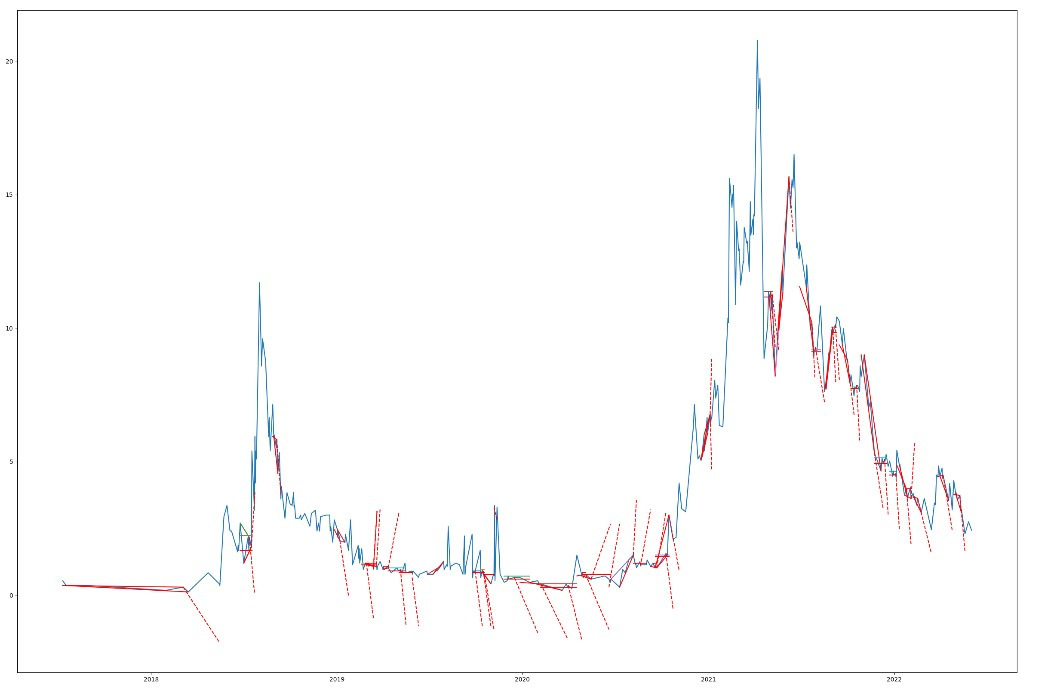
\includegraphics[width=0.8\textwidth]{pic/GBOX.jpg}
        \caption{График акций и технические фигуры Greenbox POS}
    \end{figure}
   
    \begin{table}[!hbt]
        \centering
        \begin{tabular}{|l|c|c|c|}
        \hline
        Фигура                      & \multicolumn{1}{l|}{Количество найденных} & Совпадение & Доля  \\ \hline
        Вымпел                      & 1                                         & 1          & 0.014 \\ \hline
        Нисходящий флаг             & 1                                         & 1          & 0.014 \\ \hline
        Восходящий флаг             & 4                                         & 2          & 0.058 \\ \hline
        Прямоугольник               & 1                                         & 0          & 0.014 \\ \hline
        Нисходящий ромб             & 0                                         & 0          & 0     \\ \hline
        Восходящий ромб             & 0                                         & 0          & 0     \\ \hline
        Голова и плечи              & 1                                         & 1          & 0.014 \\ \hline
        Перевернутые голова и плечи & 4                                         & 1          & 0.058 \\ \hline
        \end{tabular}
        \end{table}

    Ввиду развития технологий электронных платежей с использованием \\блокчейна,
    рассмотрим котировки компании Greenbox POS "--- одной из самых волатильных 
    акций в данной сфере.

    Для данной акции, за весь рассматриваемый период технический анализ 
    представляется возможным. В большинстве случаев предполагаемый курс совпал с 
    действительным.
    
    Котировка считается технически анализируемой.

    Теперь перейдем к анализу акций с низкой волатильностью.

    \subsubsection{Campbell Soup Company}
    
    \begin{figure}[H]
        \centering
        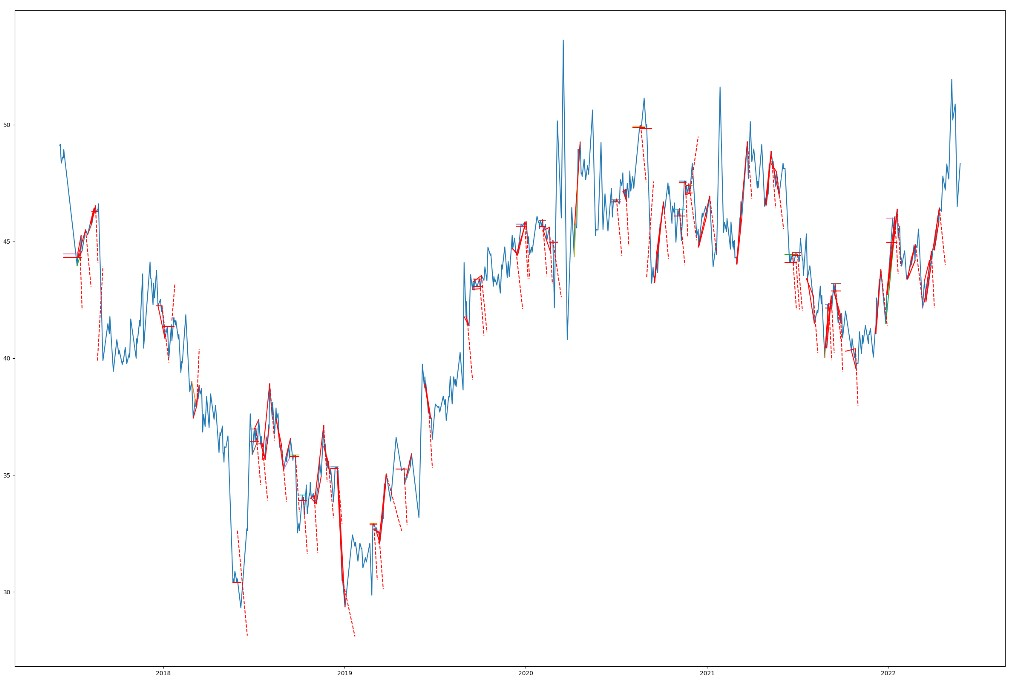
\includegraphics[width=0.8\textwidth]{pic/CPB.jpg}
        \caption{График акций и технические фигуры Campbell Soup Company}
    \end{figure}
   
    \begin{table}[!hbt]
        \centering
        \begin{tabular}{|l|c|c|c|}
        \hline
        Фигура                      & \multicolumn{1}{l|}{Количество найденных} & Совпадение & Доля  \\ \hline
        Вымпел                      & 1                                         & 1          & 0.01  \\ \hline
        Нисходящий флаг             & 0                                         & 0          & 0     \\ \hline
        Восходящий флаг             & 14                                        & 14         & 0.136 \\ \hline
        Прямоугольник               & 1                                         & 1          & 0.01  \\ \hline
        Нисходящий ромб             & 0                                         & 0          & 0     \\ \hline
        Восходящий ромб             & 0                                         & 0          & 0     \\ \hline
        Голова и плечи              & 4                                         & 4          & 0.039 \\ \hline
        Перевернутые голова и плечи & 1                                         & 1          & 0.01  \\ \hline
        \end{tabular}
        \end{table}

    
    Campbell Soup Company (также известная как Campbell's) "--- американская 
    компания, являющаяся крупнейшим в мире производителем консервированных 
    супов.
    
    Стоит сказать, что для данной акции всего было найдено 103 технические
    фигуры за рассматриваемый период, что свидетельствует о возможности
    технического анализа. В сводной таблице же приведены рассматриваемые в 
    данной работе только те технические фигуры, смысл рассматривать которые
    есть, так как другие фигуры технического анализа не являются эталонными
    для рассмотрения.
    
    Для данной акции, за весь рассматриваемый период технический анализ 
    представляется возможным. В большинстве случаев предполагаемый курс совпал с 
    действительным.
    
    Котировка считается технически анализируемой.

    \subsubsection{Johnson and Johnson}
    
    \begin{figure}[H]
        \centering
        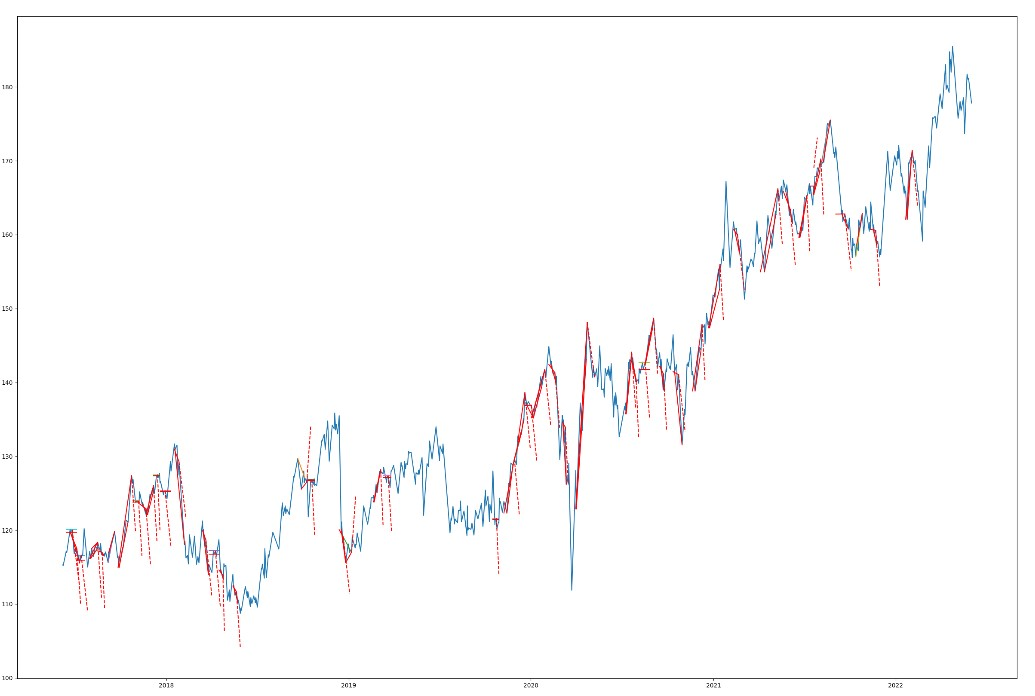
\includegraphics[width=0.8\textwidth]{pic/JNJ.jpg}
        \caption{График акций и технические фигуры Johnson and Johnson}
    \end{figure}
   
    \begin{table}[!hbt]
        \centering
        \begin{tabular}{|l|c|c|c|}
        \hline
        Фигура                      & \multicolumn{1}{l|}{Количество найденных} & Совпадение & Доля  \\ \hline
        Вымпел                      & 2                                         & 2          & 0.025 \\ \hline
        Нисходящий флаг             & 0                                         & 0          & 0     \\ \hline
        Восходящий флаг             & 6                                         & 6          & 0.076 \\ \hline
        Прямоугольник               & 0                                         & 0          & 0     \\ \hline
        Нисходящий ромб             & 0                                         & 0          & 0     \\ \hline
        Восходящий ромб             & 0                                         & 0          & 0     \\ \hline
        Голова и плечи              & 0                                         & 0          & 0     \\ \hline
        Перевернутые голова и плечи & 1                                         & 1          & 0.013 \\ \hline
        \end{tabular}
        \end{table}

    
        Johnson and Johnson "--- американская холдинговая компания, возглавляющая
        группу из более чем 250 дочерних компаний по всему миру, производящих
        лекарственные препараты, санитарно-гигиенические товары и медицинское
        оборудование.
    
        Исходя из полученных данных, можно сделать вывод, что акции не относятся
        к техничным. Из рассматриваемых фигур не были найдены: <<Нисходящий 
        флаг>>, <<Прямоугольник>>, <<Ромб>>, <<Голова и плечи>>.

        Котировка не считается технически анализируемой.

        \subsubsection{Altria Group}
    
        \begin{figure}[H]
            \centering
            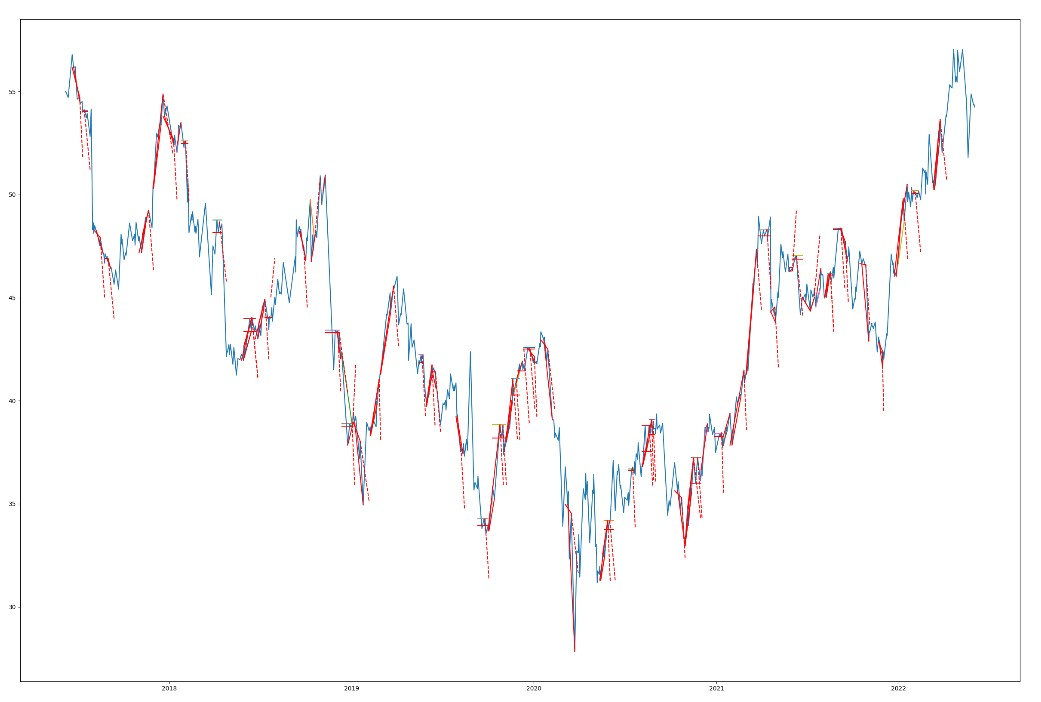
\includegraphics[width=0.8\textwidth]{pic/MO.jpg}
            \caption{График акций и технические фигуры Altria Group}
        \end{figure}
       
        \begin{table}[!hbt]
            \centering
            \begin{tabular}{|l|c|c|c|}
            \hline
            Фигура                      & \multicolumn{1}{l|}{Количество найденных} & Совпадение & Доля  \\ \hline
            Вымпел                      & 2                                         & 2          & 0.018 \\ \hline
            Нисходящий флаг             & 0                                         & 0          & 0     \\ \hline
            Восходящий флаг             & 17                                        & 17         & 0.153 \\ \hline
            Прямоугольник               & 0                                         & 0          & 0     \\ \hline
            Нисходящий ромб             & 1                                         & 1          & 0.009 \\ \hline
            Восходящий ромб             & 0                                         & 0          & 0     \\ \hline
            Голова и плечи              & 1                                         & 1          & 0.009 \\ \hline
            Перевернутые голова и плечи & 1                                         & 1          & 0.009 \\ \hline
            \end{tabular}
            \end{table}
    
        
            Altria Group "--- один из лидеров мирового рынка табачных изделий, 
            который является материнской компанией таких производителей сигарет, 
            как Philip Morris USA, John Middleton и U.S. Smokeless Tobacco 
            Company.
    
        
        Для данной акции всего было найдено 111 технических фигур за 
        рассматриваемый период, что свидетельствует о возможности технического 
        анализа. Информация о фигурах, представляющих интерес представлена в 
        таблице.
        
        Для данной акции, за весь рассматриваемый период технический анализ 
        представляется возможным. В большинстве случаев предполагаемый курс 
        совпал с действительным.
        
        Котировка считается технически анализируемой.

        \subsubsection{Sprouts Farmers Market}
    
        \begin{figure}[H]
            \centering
            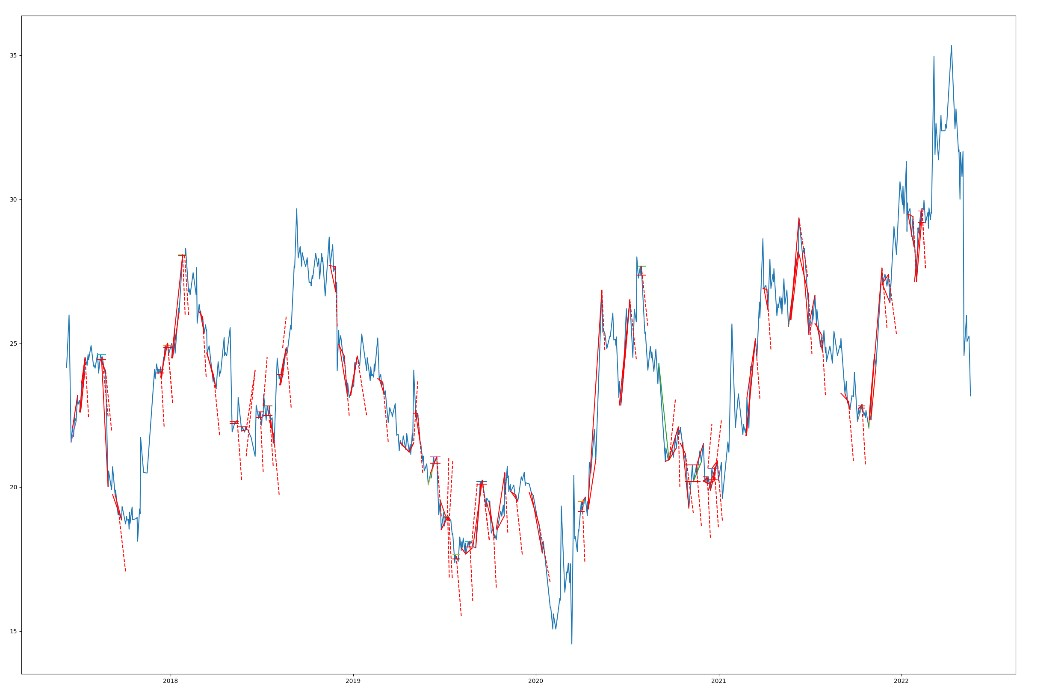
\includegraphics[width=0.8\textwidth]{pic/SFM.jpg}
            \caption{График акций и технические фигуры Sprouts Farmers Market}
        \end{figure}
       
        \begin{table}[!hbt]
            \centering
            \begin{tabular}{|l|c|c|c|}
            \hline
            Фигура                      & \multicolumn{1}{l|}{Количество найденных} & Совпадение & Доля  \\ \hline
            Вымпел                      & 2                                         & 2          & 0.017 \\ \hline
            Нисходящий флаг             & 1                                         & 1          & 0.009 \\ \hline
            Восходящий флаг             & 15                                        & 15         & 0.128 \\ \hline
            Прямоугольник               & 0                                         & 0          & 0     \\ \hline
            Нисходящий ромб             & 0                                         & 0          & 0     \\ \hline
            Восходящий ромб             & 3                                         & 3          & 0.026 \\ \hline
            Голова и плечи              & 0                                         & 0          & 0     \\ \hline
            Перевернутые голова и плечи & 4                                         & 4          & 0.034 \\ \hline
            \end{tabular}
            \end{table}
    
        
            Sprouts Farmers Market "--- сеть супермаркетов, специализирующаяся 
            на свежих, натуральных и органических продуктах.
    
        
        Для данной акции всего было найдено 117 технических фигур за 
        рассматриваемый период, что свидетельствует о возможности технического 
        анализа. Информация о фигурах, представляющих интерес представлена в 
        таблице.
        
        Для данной акции, за весь рассматриваемый период технический анализ 
        представляется возможным. В большинстве случаев предполагаемый курс 
        совпал с действительным.
        
        Котировка считается технически анализируемой.

        Теперь перейдем к анализу котировок криптовалют. Для начала возьмем в
        качестве анализируемой акции одну из самых популярных валют "--- 
        Bitcoin. Затем наоборот возьмем для анализа не самую популярную валюту
        "--- EOS.

        \subsubsection{Bitcoin}
    
        \begin{figure}[H]
            \centering
            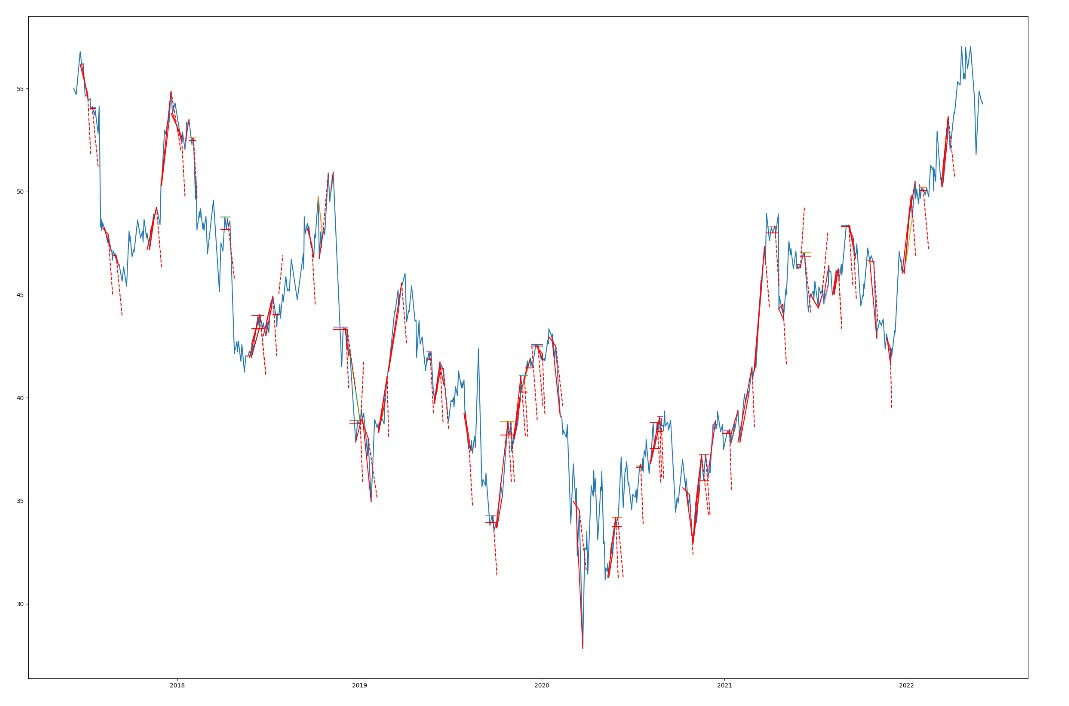
\includegraphics[width=0.8\textwidth]{pic/BTC.jpg}
            \caption{График акций и технические фигуры Bitcoin}
        \end{figure}
       
        \begin{table}[!hbt]
            \centering
            \begin{tabular}{|l|c|c|c|}
            \hline
            Фигура                      & \multicolumn{1}{l|}{Количество найденных} & Совпадение & Доля  \\ \hline
            Вымпел                      & 1                                         & 1          & 0.013 \\ \hline
            Нисходящий флаг             & 1                                         & 1          & 0.013 \\ \hline
            Восходящий флаг             & 2                                         & 2          & 0.026 \\ \hline
            Прямоугольник               & 3                                         & 3          & 0.039 \\ \hline
            Нисходящий ромб             & 1                                         & 1          & 0.013 \\ \hline
            Восходящий ромб             & 1                                         & 1          & 0.013 \\ \hline
            Голова и плечи              & 5                                         & 5          & 0.065 \\ \hline
            Перевернутые голова и плечи & 5                                         & 5          & 0.065 \\ \hline
            \end{tabular}
            \end{table}
        
        Bitcoin является самой популярной криптовалютой в мире.

        Для данной акции всего было найдено 77 технических фигур за 
        рассматриваемый период, что свидетельствует о возможности технического 
        анализа. Информация о фигурах, представляющих интерес представлена в 
        таблице.
        
        Для данной акции, за весь рассматриваемый период технический анализ 
        представляется возможным. В большинстве случаев предполагаемый курс 
        совпал с действительным.
        
        Котировка считается технически анализируемой.

        \subsubsection{EOS}
    
        \begin{figure}[H]
            \centering
            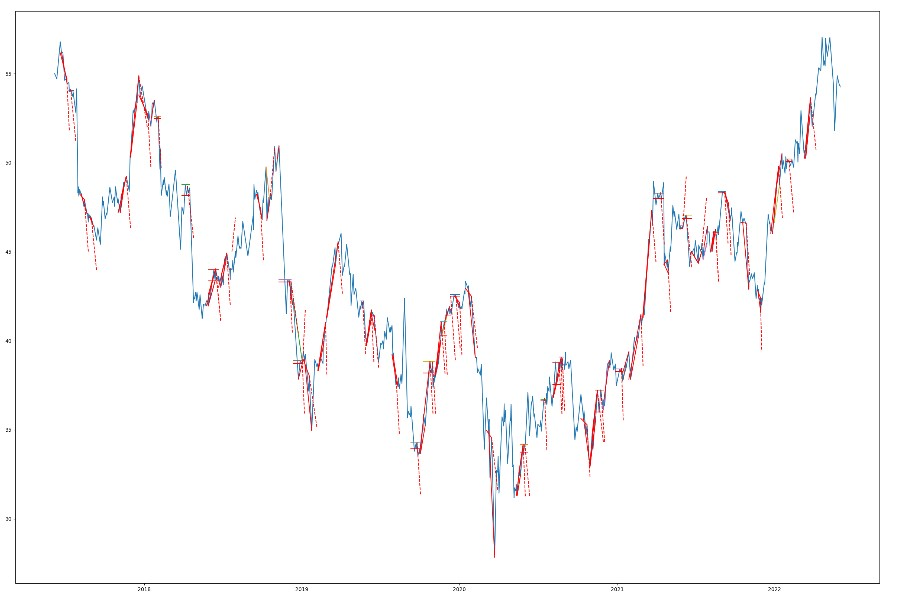
\includegraphics[width=0.8\textwidth]{pic/EOS.jpg}
            \caption{График акций и технические фигуры EOS}
        \end{figure}
       
        \begin{table}[!hbt]
            \centering
            \begin{tabular}{|l|c|c|c|}
            \hline
            Фигура                      & \multicolumn{1}{l|}{Количество найденных} & Совпадение & Доля  \\ \hline
            Вымпел                      & 1                                         & 1          & 0.004 \\ \hline
            Нисходящий флаг             & 1                                         & 1          & 0.004 \\ \hline
            Восходящий флаг             & 24                                        & 23         & 0.09  \\ \hline
            Прямоугольник               & 8                                         & 8          & 0.03  \\ \hline
            Нисходящий ромб             & 3                                         & 3          & 0.011 \\ \hline
            Восходящий ромб             & 1                                         & 1          & 0.004 \\ \hline
            Голова и плечи              & 13                                        & 13         & 0.049 \\ \hline
            Перевернутые голова и плечи & 11                                        & 11         & 0.041 \\ \hline
            \end{tabular}
            \end{table}
        
        Для данной акции всего было найдено 266 технических фигур за 
        рассматриваемый период и является максимальным количеством из
        рассматриваемых.
        
        Для данной акции, за весь рассматриваемый период технический анализ 
        представляется возможным. В большинстве случаев предполагаемый курс 
        совпал с действительным.
        
        Котировка считается технически анализируемой.
\conclusion

    В данной работе были рассмотрены детерминированные методы поиска технических
    фигур на курсах акций. Проведен анализ работы алгоритма на акциях с высокой
    волатильностью и низкой, а также на акциях криптовалют. Алгоритм в некоторых
    случаях может работать некорректно в следствие неправильной подобранных
    значений допуска $\varepsilon$ в фигурах, где это значение используется.
    Также были рассмотрены теоретические основы нейросетей, описаны основные
    принципы работы и их роль в решении, основы технического анализа и основные
    определения трейдинга. 

    В качестве практической части работы была описана программная реализация
    алгоритма поиска технических фигур на акциях, получение статистики по
    фигурам, а также отрисовка данных фигур на графике акции с предполагаемым
    ростом или падением курса.


    \bibliographystyle{gost780uv}
    \inputencoding{cp1251}
    \bibliography{thesis}
    \inputencoding{utf8}

\appendix
    \setminted[py]{fontsize=\small, breaklines=true, style=bw, linenos}
    \section{Код \texttt{drawing.py}}
    \inputminted{py}{code/drawing.py}

    \section{Код \texttt{figures.py}}
    \inputminted{py}{code/figures.py}

    \section{Код \texttt{main.py}}
    \inputminted{py}{code/main.py}

\end{document}
